% NTCIR-19 CAMEO poster --- team retrank --- A0 portrait
% Every number and claim here is taken from the submitted paper
% (docs/paper/ntcir19_cameo_retrank.tex); do not add results that are not in it.
\documentclass[25pt, a0paper, portrait, margin=0mm, innermargin=18mm,
               blockverticalspace=10mm, colspace=14mm, subcolspace=8mm]{tikzposter}
\usepackage{booktabs}
\usepackage{array}
\usepackage{amsmath}
\usepackage{graphicx}
\usepackage{tikz}
\usetikzlibrary{arrows.meta,positioning,fit,calc}

\definecolor{accent}{RGB}{0,96,160}
\definecolor{accentdk}{RGB}{0,60,105}
\definecolor{lightgray}{RGB}{242,244,247}

\usetheme{Default}
\usecolorstyle[colorOne=accent,colorTwo=accentdk,colorThree=lightgray]{Denmark}
% readable block titles: white on dark blue
\colorlet{blocktitlebgcolor}{accentdk}
\colorlet{blocktitlefgcolor}{white}
\colorlet{blockbodybgcolor}{white}
\colorlet{blockbodyfgcolor}{black}
\tikzposterlatexaffectionproofoff

\newcommand{\callout}[1]{%
  \coloredbox[bgcolor=lightgray,fgcolor=black,framecolor=accent,linewidth=2pt]{#1}}

\settitle{
  \centering
  \color{white}
  {\bfseries\Huge Metadata-Grounded Composed Image Retrieval for Vietnamese E-commerce\par}
  \vspace{8mm}
  {\LARGE A Structured-Attribute and Local-VLM Reranking Pipeline\par}
  \vspace{12mm}
  {\Large \textbf{Alessandro Magnani} \;$\cdot$\; Independent \;$\cdot$\; Team \textbf{retrank} \;$\cdot$\; ale.magnani@gmail.com\par}
  \vspace{4mm}
  {\large NTCIR-19 CAMEO --- Composed Image Retrieval (CIR) Subtask \quad$\cdot$\quad Tokyo, December 2026\par}
}

\begin{document}
\maketitle[width=800mm]

%% ===================== ROW 1: TASK | APPROACH =====================
\begin{columns}
\column{0.34}

\block{The Task}{
Given a \textbf{reference product image} and a \textbf{natural-language
modification}, rank a fixed catalogue.
\begin{itemize}
  \item \textbf{Corpus:} 4{,}086 Vietnamese skincare products (cleansers,
        toners, sunscreens, and more), each with an image, brand, numeric
        price (VND) and translated name/description.
  \item \textbf{Queries:} 20 official CIR topics --- Vietnamese shopper
        requests, e.g.\ \emph{``the same product but cheaper''},
        \emph{``a gel cleanser from brand X''}.
  \item \textbf{Judging:} pooled across teams, 3-point human relevance;
        nDCG@5 / nDCG@10.
\end{itemize}
\callout{\textbf{Why it is hard here:} many requests are about
\emph{price, brand, format} --- attributes that live in the product's text
metadata and are invisible to a purely visual encoder.}
}

\column{0.66}

\block{Approach: a Two-Stage Pipeline}{
\centering
\resizebox{\linewidth}{!}{%
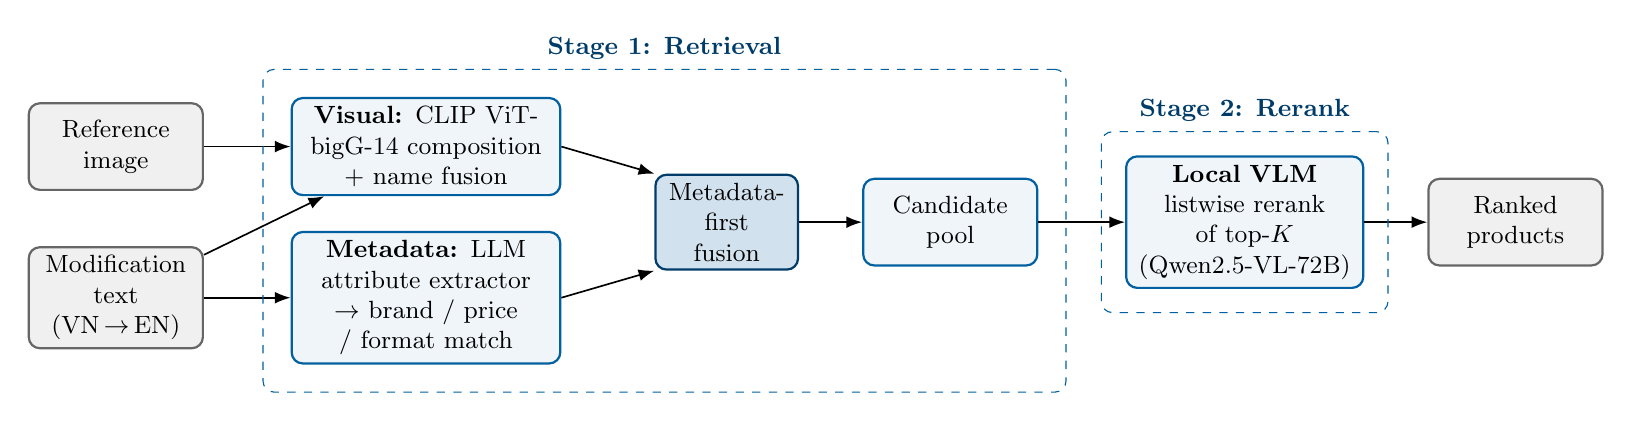
\begin{tikzpicture}[
  font=\fontsize{9}{11}\selectfont,
  box/.style={draw=accent, thick, rounded corners, align=center, minimum height=11mm,
              text width=3.2cm, inner sep=3pt, fill=accent!6},
  io/.style={draw=black!60, thick, rounded corners, align=center, minimum height=11mm,
             text width=2.0cm, inner sep=3pt, fill=black!6},
  op/.style={draw=accentdk, thick, rounded corners, align=center, minimum height=11mm,
             text width=1.6cm, inner sep=3pt, fill=accent!18},
  arr/.style={-{Latex[length=2mm]}, semithick},
]
  \node[io] (img) {Reference image};
  \node[io, below=7mm of img] (txt) {Modification text (VN\,$\to$\,EN)};
  \node[box, right=11mm of img] (visual)
        {\textbf{Visual:} CLIP ViT-bigG-14 composition + name fusion};
  \node[box, right=11mm of txt] (meta)
        {\textbf{Metadata:} LLM attribute extractor $\to$ brand / price / format match};
  \node[op] (fuse) at ($(visual.east)!0.5!(meta.east) + (2.1cm,0)$) {Metadata-first fusion};
  \node[box, right=8mm of fuse, text width=2.0cm] (pool) {Candidate pool};
  \node[box, right=11mm of pool, text width=2.8cm] (rerank)
        {\textbf{Local VLM} listwise rerank of top-$K$ (Qwen2.5-VL-72B)};
  \node[io, right=8mm of rerank] (out) {Ranked products};
  \draw[arr] (img) -- (visual);
  \draw[arr] (txt) -- (visual);
  \draw[arr] (txt) -- (meta);
  \draw[arr] (visual.east) -- (fuse.north west);
  \draw[arr] (meta.east) -- (fuse.south west);
  \draw[arr] (fuse) -- (pool);
  \draw[arr] (pool) -- (rerank);
  \draw[arr] (rerank) -- (out);
  \node[draw=accent, dashed, rounded corners, inner sep=3.5mm,
        fit=(visual)(meta)(fuse)(pool),
        label={[font=\fontsize{9}{11}\selectfont\bfseries, text=accentdk]above:Stage 1: Retrieval}] {};
  \node[draw=accent, dashed, rounded corners, inner sep=3mm,
        fit=(rerank),
        label={[font=\fontsize{9}{11}\selectfont\bfseries, text=accentdk]above:Stage 2: Rerank}] {};
\end{tikzpicture}}
\vspace{4mm}

\raggedright
\begin{minipage}[t]{0.49\linewidth}
\begin{itemize}
  \item \textbf{Visual branch:} training-free composition
        $q=\mathrm{norm}(\hat e_\text{img}+\hat e_\text{txt})$; each product
        vector fuses its image and product-name embeddings ($a{=}0.2$).
        Exhaustive search, no ANN.
  \item \textbf{Fusion:} metadata hits first, then the visual list.
\end{itemize}
\end{minipage}\hfill
\begin{minipage}[t]{0.49\linewidth}
\begin{itemize}
  \item \textbf{Metadata branch:} an LLM (Claude Haiku) reads the request text
        and extracts the target brand, price, format, claim. Brand-matched
        products are scored by format/claim keyword hits $+$ Gaussian price
        proximity ($\sigma{=}0.4$); \emph{abstains} if no confident brand.
  \item \textbf{Stage 2:} a local open-weight VLM (vLLM) reorders the top-$K$
        ($K{=}20$) against the reference image $+$ request.
\end{itemize}
\end{minipage}
}

\end{columns}

%% ===================== ROW 2 =====================
\begin{columns}

%% --------------------- COLUMN 1 ---------------------
\column{0.33}

\block{Three Evaluation Regimes}{
Our numbers come from three ground truths that are \textbf{not comparable}:
\vspace{3mm}
\begin{center}
\begin{tabular}{@{}>{\raggedright\arraybackslash}p{0.25\linewidth}>{\raggedright\arraybackslash}p{0.36\linewidth}>{\raggedright\arraybackslash}p{0.28\linewidth}@{}}
\toprule
Regime & Ground truth & Used for \\ \midrule
\textbf{Dev-429} (ours) & synthetic, one exact answer per query & Stage-1 recall (harsh) \\
\addlinespace
\textbf{Official-20 proxy} & Claude Sonnet vision judge over our runs; one pass & sanity check (lenient, noisy) \\
\addlinespace
\textbf{Official} & pooled human judgments & the score that counts \\
\bottomrule
\end{tabular}
\end{center}
\vspace{2mm}
Dev-429: five templated rules (\emph{cheaper}/\emph{pricier} same brand;
\emph{format}/\emph{brand}/\emph{claim} swap). Low Dev vs.\ high proxy scores
reflect the metric, not the system. Never tuned on official queries.
}

\block{Finding 1 --- Recall Is the Ceiling}{
A reranker can only reorder what Stage-1 retrieved. With one gold answer per
Dev query, the best nDCG@10 \emph{any} reranker can reach over a fixed pool
equals that pool's \textbf{recall} at its depth.
\vspace{3mm}
\begin{center}
\resizebox{\linewidth}{!}{%
\begin{tabular}{@{}lccc@{}}
\toprule
Stage-1 pool (Dev-429) & R@20 & R@50 & Stage-1 nDCG@10 \\
\midrule
SEARLE-Phi                     & 0.084 & 0.154 & 0.029 \\
bigG $+$ name fusion (visual)  & 0.359 & 0.436 & 0.157 \\
\textbf{Metadata-fused}        & \textbf{0.431} & \textbf{0.527} & \textbf{0.200} \\
\bottomrule
\end{tabular}}
\end{center}
\vspace{2mm}
Visual backbones plateau near 0.44 R@50; only metadata fusion breaks it.
On the SEARLE-Phi pool a \emph{perfect} reranker still misses $>$84\% of
queries.
\callout{Improving Stage-1 raises the ceiling; reranker tuning only closes the
gap beneath it.}
}

\block{What Did Not Work}{
\begin{itemize}
  \item \textbf{RRF} of CLIP backbones; \textbf{query rewriting}: no gain.
  \item \textbf{Brand in the embedding} / high name-fusion weight: worse
        than symbolic brand matching.
  \item \textbf{Format/claim as hard filters:} the pool collapses.
  \item \textbf{Visually reranking the metadata pool:} Dev 0.200$\to$0.173
        in one run --- a caution; mechanism unverified.
  \item \textbf{MagicLens:} environment blocked, not measured.
\end{itemize}
}

%% --------------------- COLUMN 2 ---------------------
\column{0.34}

\block{Finding 2 --- Price Carries the Metadata Gain}{
Metadata-only ranking, gold fields, one term at a time (Dev, nDCG@10):
\vspace{3mm}
\begin{center}
\begin{tabular}{@{}lc@{}}
\toprule
Terms enabled & nDCG@10 \\ \midrule
brand only               & 0.084 \\
brand $+$ format         & 0.110 \\
brand $+$ claim          & 0.088 \\
\textbf{brand $+$ price} & \textbf{0.232} \\
all four terms           & 0.211 \\
\bottomrule
\end{tabular}
\end{center}
\vspace{2mm}
\begin{itemize}
  \item Price carries almost all the gain; format/claim bonuses are net noise.
  \item LLM extraction is lossless on the templated price rules, but was not
        validated on natural official queries; overall Dev 0.131 (extracted)
        vs.\ 0.211 (gold).
  \item \textbf{Complementary, not universal:} on the full 2{,}083-query Dev
        set (79\% free-form) fusion is roughly neutral (0.115 vs.\ 0.119).
\end{itemize}
}

\block{Finding 3 --- Local VLM Rerankers Are Competitive with a Hosted API}{
Same SEARLE-Phi top-20 pool, Official-20 proxy judge:
\vspace{3mm}
\begin{center}
\resizebox{\linewidth}{!}{%
\begin{tabular}{@{}lcc@{}}
\toprule
Reranker & proxy nDCG@10 & marginal cost/pass \\ \midrule
Qwen2.5-VL-72B (local)    & \textbf{0.913} & $\sim$\$0 \\
InternVL3-38B (local)     & 0.907 & $\sim$\$0 \\
Qwen2.5-VL-32B (local)    & 0.894 & $\sim$\$0 \\
Haiku (hosted API)        & 0.872 & $\sim$\$11 \\
Pixtral-Large (local)     & 0.869 & $\sim$\$0 \\
\bottomrule
\end{tabular}}
\end{center}
\vspace{2mm}
Three of four local models score above the API, but the gaps are within proxy
noise. $\sim$\$0 is the \emph{marginal} cost once a GPU is rented --- which made
a 21-configuration LLM-guided search affordable.
}

\block{Implementation \& Cost}{
\begin{itemize}
  \item open\_clip ViT-bigG/14 (\texttt{laion2b\_s39b\_b160k}); corpus
        embeddings cached; exhaustive cosine search.
  \item Extractor: Claude Haiku, per-query cached. Rerankers: vLLM on rented
        dual-A100 hosts.
  \item Total spend: $\sim$\$235 hosted-LLM API (early reranking, Dev
        generation, proxy judge, extractor) $+$ $\sim$\$60 GPU.
\end{itemize}
}

%% --------------------- COLUMN 3 ---------------------
\column{0.33}

\block{Official Results}{
\begin{center}
\resizebox{\linewidth}{!}{%
\begin{tabular}{@{}llcc@{}}
\toprule
Run & Stage-1 $\to$ reranker & @5 & @10 \\ \midrule
\textbf{Run1} & \textbf{fused (bigG+meta) $\to$ Qwen-72B}  & \textbf{0.740} & \textbf{0.714} \\
Run5 & bigG name-fused$+$BU $\to$ Qwen-32B    & 0.739 & 0.709 \\
Run2 & SEARLE-Phi $\to$ Qwen-72B              & 0.680 & 0.636 \\
Run3 & SEARLE-Phi $\to$ InternVL3-38B         & 0.650 & 0.628 \\
Run4 & SEARLE-Phi $\to$ Qwen-32B              & 0.625 & 0.606 \\
\bottomrule
\end{tabular}}
\end{center}
{\small nDCG on 20 topics, pooled human judgments. BU = symbolic brand-union.\par}
\vspace{2mm}
\begin{itemize}
  \item \textbf{3rd of 5 teams} (15 runs) at both cutoffs. At nDCG@10 the
        top four lie within \textbf{0.019} --- no ordering inferred among
        2nd--4th.
  \item \textbf{Same pool, three rerankers} (Runs 2--4): only
        \textbf{0.030} nDCG@10 apart (Friedman $p{\approx}0.52$) --- yet
        per-topic ranges reach 0.22.
  \item \textbf{Same reranker, new Stage-1 pool:} Run2$\to$Run1
        \textbf{$+$0.078} and Run4$\to$Run5 \textbf{$+$0.103} nDCG@10.
\end{itemize}
\callout{In aggregate, \textbf{candidate generation is the larger lever}. The
contrasts swap the whole Stage-1 family (Run5's brand-union added no official
candidates), so metadata's own effect is shown on Dev.}
}

\block{Where It Still Fails}{
Metadata-fused Stage-1 per rule (Dev, nDCG@10, extracted fields):
\vspace{2mm}
\begin{center}
\begin{tabular}{@{}ccccc@{}}
\toprule
cheaper & pricier & format & claim & brand swap \\ \midrule
0.293 & 0.362 & 0.234 & 0.173 & \textbf{0.117} \\
\bottomrule
\end{tabular}
\end{center}
\vspace{2mm}
\begin{itemize}
  \item \textbf{Brand swap} is the weakest rule, gated by brand-name resolution.
  \item \textbf{Official price-band topics} (Run1): 0.586 vs.\ 0.870 nDCG@10
        (11 vs.\ 9). Recall is not lower: an \emph{ordering} gap; descriptive.
\end{itemize}
}

\block{Takeaways}{
\begin{itemize}
  \item \textbf{Recall, not reranking,} caps CIR on a structured e-commerce
        corpus --- in aggregate; single topics can still be reranker-sensitive.
  \item \textbf{Structured metadata --- especially price ---} recovers what a
        visual encoder cannot see; gains concentrate on structured requests.
  \item \textbf{Local open-weight VLM rerankers} are competitive with a hosted
        API at near-zero marginal cost.
  \item \textbf{Next:} brand resolution; re-audit metadata-pool reranking;
        validate extraction on natural queries.
\end{itemize}
}

\end{columns}
\end{document}
